\documentclass[conference]{IEEEtran}
\IEEEoverridecommandlockouts
\usepackage{cite}
\usepackage{amsmath,amssymb,amsfonts}
\usepackage{graphicx}
\usepackage{textcomp}
\usepackage{xcolor}
\usepackage{booktabs}
\usepackage{url}

\begin{document}

\title{Smart Tourist Safety Monitoring and Incident Response System Using AI, Geo-Fencing, and Blockchain-Based Digital Identity}

\author{
\IEEEauthorblockN{Ajay K}
\IEEEauthorblockA{\textit{Dept. of Computer Science and Engineering} \\
\textit{K. S. Rangasamy College of Technology (Autonomous)}\\
Tiruchengode, Tamil Nadu, India \\
ajaykannan176@gmail.com}
\and
\IEEEauthorblockN{Ashwika K}
\IEEEauthorblockA{\textit{Dept. of Computer Science and Engineering} \\
\textit{K. S. Rangasamy College of Technology (Autonomous)}\\
Tiruchengode, Tamil Nadu, India \\
ashwikakuppusamy@gmail.com}
\and
\IEEEauthorblockN{Dr. B. G. Geetha}
\IEEEauthorblockA{\textit{Professor, Dept. of Computer Science and Engineering} \\
\textit{K. S. Rangasamy College of Technology (Autonomous)}\\
Tiruchengode, Tamil Nadu, India \\
geetha@ksrct.ac.in}
}

\maketitle

\begin{abstract}
Visitors travelling in unfamiliar destinations face medical emergencies, theft, disorientation, and restricted-area hazards. When identity checks, location tracking, and emergency reporting live in separate tools, responders lose critical minutes gathering context. This paper presents the six-module implementation and controlled evaluation of a Smart Tourist Safety Monitoring and Incident Response System. The prototype connects a Kotlin Jetpack Compose Android app, a Python FastAPI backend with a PostgreSQL/PostGIS spatial schema and WebSocket streaming, circular and polygonal geo-fencing, movement-window anomaly detection, Ed25519-signed Verifiable Credentials anchored on a local hash-chained permissioned ledger (with companion Hyperledger Fabric chaincode), and a React/OpenStreetMap authority console. Personal records remain off-chain while SHA-256 credential hashes, issuer public keys, expiry timestamps, and revocation flags are recorded on-chain. We separate trajectory-split simulation tests (Experiments A, B, and feature ablation across 10 independent seeds) from implemented software benchmarks (Experiments C and D). Across 10 seeds (300 held-out trajectories per seed at 3.5~m GPS noise), Local Outlier Factor (LOF) and Isolation Forest achieved F1-scores of $0.9956 \pm 0.0032$ and $0.9677 \pm 0.0110$ (0.09 and 0.66 false alerts per tourist-hour), outperforming a static rule baseline ($0.5108 \pm 0.0267$). Hybrid geo-fencing plus Isolation Forest scored $0.9672 \pm 0.0117$ F1, trading minor boundary recall for explicit restricted-zone escalation. Raising GPS error to 10--15~m or injecting 15\% jump spikes sharply increased false alerts, motivating pre-filtering before feature extraction. On the implemented backend, credential verification rejected 100\% of tampered, expired, revoked, rogue-signed, and replayed credentials in under 0.45~ms, and live WebSocket alert delivery averaged 137.37~ms across 20 end-to-end incident workflows.
\end{abstract}

\begin{IEEEkeywords}
Tourist safety, geo-fencing, blockchain, decentralised identifier, verifiable credentials, Isolation Forest, FastAPI, incident response.
\end{IEEEkeywords}

\section{Introduction}
Travellers entering unfamiliar regions often lack local contacts, hazard awareness, and rapid ways to share verified identity and location details during an emergency \cite{aliperti2020,chiranjeevi2026}. Standard help desks, patrol units, and basic SOS apps still expect the tourist to recognize danger early, keep a working data connection, and manually provide documents or coordinates. Paper ID checks are slow and easy to misplace, while storing passport scans in a single centralized database creates an attractive target for unauthorized access.

Following our earlier Phase-I system design, we built and tested a working six-module prototype that ties identity verification, spatial zone monitoring, movement anomaly scoring, and incident handling into one workflow. First, an authorized verifier issues an Ed25519-signed Verifiable Credential (VC) whose SHA-256 digest and revocation state sit on a permissioned ledger while personal fields stay off-chain. Second, a geo-fencing service checks incoming GPS fixes against safe, caution, and restricted zones with configurable warning buffers. Third, an unsupervised movement model scores speed, stop duration, and route deviation over recent time windows. Fourth, alerts from SOS presses, restricted-zone entries, or anomaly flags stream over WebSockets to an authority map dashboard, where responders acknowledge, track, and close incidents.

To avoid mixing synthetic benchmarks with live software metrics, we report our evaluation in two distinct groups. Experiments A, B, and our feature-ablation study test anomaly models and GPS noise sensitivity on synthetic trajectories split strictly by tourist ID across 10 independent seeds so adjacent windows never leak across training, validation, and test sets. Experiments C and D measure real cryptographic checks, tamper and replay rejection, WebSocket notification delay, and concurrent API throughput on the running FastAPI service. In keeping with safe decision support, an AI flag is treated as a prompt for human review rather than proof of an emergency.

Rather than claiming an unprecedented AI-blockchain paradigm, this paper makes five concrete engineering and empirical contributions: (1) a reproducible trajectory-split simulation framework for tourist safety incident scenarios; (2) a 10-seed statistical and feature-ablation comparison of Rule-Based, LOF, Isolation Forest, and hybrid geo-fencing + Isolation Forest detectors; (3) a controlled investigation of geo-fence and anomaly sensitivity under 2--15~m GPS error, 30\% packet dropout, and 15\% jump spikes; (4) an experimental analysis demonstrating why zone-context fusion trades minor boundary recall for explicit restricted-zone escalation; and (5) a privacy-conscious Ed25519 + SHA-256 credential-integrity prototype integrated with a six-module mobile-to-dashboard workflow.

\section{Related Work}
Existing disaster-oriented tourist apps and IoT SOS prototypes show that direct panic reporting helps when network coverage holds, yet user adoption and lack of automated context limit their reach \cite{aliperti2020,chiranjeevi2026}. Regional tourism risk studies apply interpretable machine learning and deep neural models to map area-wide crime or terrain hazards \cite{george2024,premananthan2024,li2026,josephi2026,hakyemez2025}. Those macro-level maps guide patrol planning, but they cannot tell whether one specific tourist has wandered off-route or stopped unexpectedly.

At the individual level, data-driven geo-fencing triggers boundary alerts \cite{sasaki2024}, and trajectory outlier surveys motivate unsupervised detectors such as Isolation Forest and Local Outlier Factor (LOF) for wearable or mobile sensor streams \cite{belhadi2020,chandola2009,ali2025}. Meanwhile, self-sovereign identity (SSI) and Hyperledger Fabric studies establish how decentralised identifiers (DIDs) and off-chain hashing protect personal data while keeping integrity verifiable \cite{mazzocca2025,muhle2018,soltani2021,figueroa2021,akhison2025,khairnar2025,mountije2025,prados2023,rana2022,zyskind2015}. Table~\ref{tab:related} contrasts these separate strands with our integrated prototype.

\begin{table}[t]
\centering
\caption{Comparison of Related Research Strands}
\label{tab:related}
\scriptsize
\begin{tabular}{@{}p{1.9cm}p{1.7cm}p{1.8cm}p{2.1cm}@{}}
\toprule
\textbf{Strand} & \textbf{Technology} & \textbf{Primary Focus} & \textbf{Gap Addressed} \\
\midrule
Safety apps \cite{aliperti2020,chiranjeevi2026} & Mobile / GPS / SOS & Manual panic alerts & Adds AI context \& DID \\
Risk maps \cite{li2026,josephi2026,hakyemez2025} & ML / spatial models & Regional / urban risk & Per-tourist live tracking \\
Geo-fencing \cite{sasaki2024} & Zone boundaries & Boundary crossing & Warning buffers + AI \\
Trajectory ML \cite{belhadi2020,ali2025} & LOF / Isolation Forest & Outlier movement & Trajectory split + GPS stress \\
SSI \& ledger \cite{mazzocca2025,figueroa2021,zyskind2015} & DID / VC / Fabric & Off-chain PII hash & Ed25519 + revocation + replay \\
Ours (Implemented) & Kotlin + FastAPI + React & 6-module workflow & Measured Exp. A--D \\
\bottomrule
\end{tabular}
\end{table}

\section{System Architecture and Implemented Modules}
Fig.~\ref{fig:arch} illustrates the six implemented modules and the data paths linking mobile telemetry, risk analysis, credential anchoring, and authority response.

\begin{figure}[t]
\centering
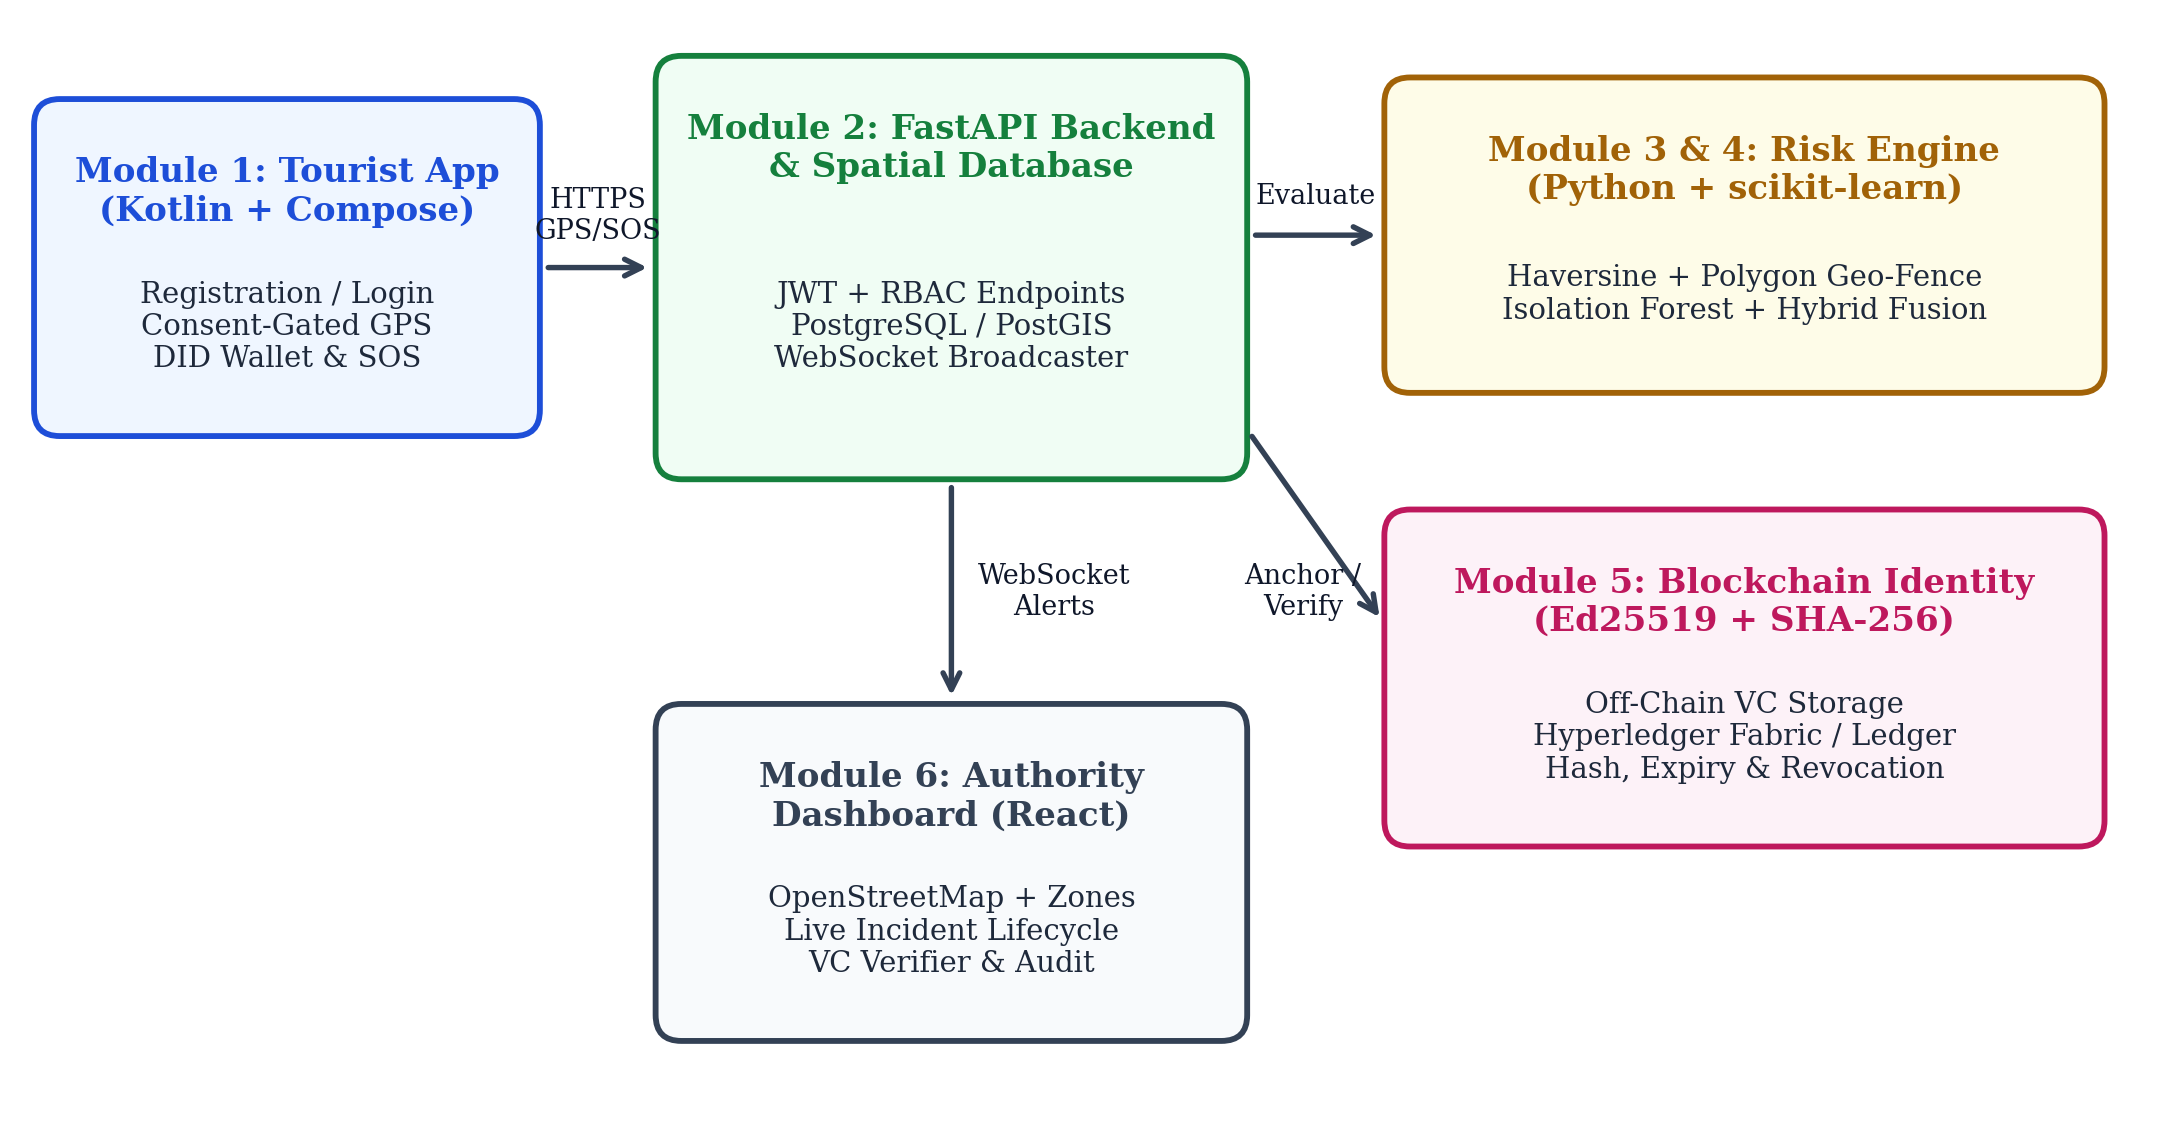
\includegraphics[width=\columnwidth]{figures/fig1_architecture.png}
\caption{Implemented six-module architecture connecting the Kotlin Android app, FastAPI/PostGIS backend, geo-fence and AI risk engine, blockchain identity module, and React/OpenStreetMap authority dashboard.}
\label{fig:arch}
\end{figure}

\subsection{Module 1: Tourist Android Application}
Built in Kotlin with Jetpack Compose (\texttt{minSdk} 26, \texttt{compileSdk} 36), the tourist app handles account registration, JWT login, DID/VC wallet viewing, consent-controlled GPS sharing via Android \texttt{LocationManager} (requiring runtime \texttt{ACCESS\_FINE\_LOCATION} approval), live safety status indicators (\texttt{safe}, \texttt{caution}, \texttt{alert}), emergency contact dialing (\texttt{Intent.ACTION\_DIAL}), and a prominent SOS button that posts critical alerts directly to the backend.

\subsection{Module 2: Backend and Spatial Database}
The API tier runs on Python 3.10, FastAPI, and SQLAlchemy 2.0. A PostgreSQL + PostGIS schema (\texttt{GEOGRAPHY} columns with GIST indexes) supports production spatial queries, while a local SQLite backend enables zero-configuration testing. Role-based access control (RBAC) separates \texttt{tourist}, \texttt{authority}, and \texttt{admin} JWT tokens, hashes passwords with PBKDF2-HMAC-SHA256, and blocks GPS ingestion whenever tracking consent is turned off.

\subsection{Modules 3 and 4: Geo-Fencing and AI Risk Engine}
The geo-fence module evaluates circular and polygonal \texttt{safe}, \texttt{caution}, and \texttt{restricted} zones, computes boundary and warning-buffer distances, and logs stateful enter/exit transitions. In parallel, the anomaly module computes seven movement features over recent observation windows and supports rule-based, LOF, Isolation Forest, and hybrid geo-fence + Isolation Forest scoring.

\subsection{Module 5: Blockchain-Based Digital Identity}
Personal details stay off-chain in \texttt{credentials\_offchain}. An authorized verifier signs canonical JSON credentials with Ed25519 and writes only the DID, credential ID, SHA-256 body hash, issuer DID, validity window, and revocation status onto a hash-chained permissioned ledger. A companion Hyperledger Fabric smart contract (\texttt{TouristIdentityContract} using \texttt{fabric-contract-api}) exposes matching \texttt{RegisterTrustedIssuer}, \texttt{AnchorCredential}, \texttt{RevokeCredential}, and \texttt{VerifyCredentialAnchor} transactions.

\subsection{Module 6: Authority Monitoring Dashboard}
Implemented in React 18, TypeScript, Vite, and Leaflet over OpenStreetMap tiles, the authority console subscribes to \texttt{/ws/authority/alerts} for live incident pushes, plots zones and priority-coded markers, creates new zones, drives status transitions (\texttt{pending}, \texttt{acknowledged}, \texttt{in\_progress}, \texttt{resolved}), and provides a credential verification and ledger inspection panel.

\section{Methodology and Algorithmic Workflow}

\subsection{Credential Integrity, Revocation, and Privacy}
For canonical JSON credential body $C$, the issuer computes $h = \text{SHA-256}(C)$ and Ed25519 signature $\sigma = \text{Sign}_{\text{sk}}(C)$. During verification of a presented credential $C'$, the verifier recomputes $h' = \text{SHA-256}(C')$ and accepts only when hash equality, trusted-issuer signature verification against the registered public key, expiration time, non-revocation on the ledger, and fresh presentation-nonce checks all pass:
\begin{equation}
h = \text{SHA-256}(C), \quad \text{Verify}(C') = [H(C') = h] \wedge \text{Sig} \wedge \text{Trust} \wedge \neg\text{Exp} \wedge \neg\text{Rev} \wedge \neg\text{Rep}.
\label{eq:vc}
\end{equation}
Because hash anchoring alone cannot establish issuer authenticity, bind a credential to its rightful holder, or prevent key misuse, our design pairs hash anchoring with trusted-issuer registration, ledger revocation flags, and one-time presentation nonces. Production deployment additionally requires hardware-backed holder key binding (e.g., Android Keystore challenge-response) and per-credential random salts inside $C$ so repeated off-chain verifications cannot be correlated across checkpoints via static on-chain hashes. Experiment C evaluates this cryptographic logic on our local hash-chained ledger; multi-node Hyperledger Fabric Raft consensus latency remains unmeasured.

\subsection{Geo-Fence Distance Evaluation}
For a circular zone centred at $(\phi_1, \lambda_1)$ with radius $r$ and warning buffer $b$, the great-circle distance $d$ to tourist position $(\phi_2, \lambda_2)$ uses the Haversine relation with mean Earth radius $R = 6{,}371{,}000\text{~m}$:
\begin{equation}
a = \sin^2\!\left(\frac{\Delta\phi}{2}\right) + \cos\phi_1 \cos\phi_2 \sin^2\!\left(\frac{\Delta\lambda}{2}\right),
\label{eq:hav_a}
\end{equation}
\begin{equation}
d = 2R\,\text{atan2}\!\left(\sqrt{a}, \sqrt{1-a}\right).
\label{eq:hav_d}
\end{equation}
Points satisfy \texttt{inside} for $d \le r$, \texttt{warning\_buffer} for $r < d \le r + b$, and \texttt{outside} otherwise. Polygonal zones apply ray-casting point-in-polygon tests paired with tangent-plane segment distance for buffers.

\subsection{Movement Features and Hybrid Anomaly Scoring}
GPS fixes with reported accuracy worse than $50\text{~m}$ are discarded. Across consecutive valid points, we extract instantaneous speed $v_i = d(p_{i-1}, p_i)/(t_i - t_{i-1})$, accumulated stop duration (displacement $< 3\text{~m}$ or $v_i < 0.35\text{~m/s}$), mean/max/standard deviation of speed, mean and max perpendicular distance to the planned route polyline, and missing-interval gap ratio:
\begin{equation}
v_i = \frac{d(p_{i-1}, p_i)}{t_i - t_{i-1}}, \quad a(x) = -\text{score\_samples}(x),
\label{eq:score}
\end{equation}
\begin{equation}
\text{Anomaly}(x) = \mathbb{I}[a(x) \ge \tau].
\label{eq:thresh}
\end{equation}
The decision threshold $\tau$ for Isolation Forest and LOF is selected via 120-point grid search on the held-out validation split to maximize F1-score, whereas the Rule-Based baseline uses fixed domain thresholds ($\text{stop} \ge 65\text{~s}$ with $\text{dev} \ge 35\text{~m}$, $\text{max\_dev} \ge 95\text{~m}$, $\text{max\_speed} \ge 4.8\text{~m/s}$, or $\text{gap\_ratio} \ge 0.5$). In the hybrid detector, restricted-zone occupancy forces an alert, caution zones and restricted buffers add $+0.06$ to $a(x)$, and safe zones subtract $0.04$ to dampen benign sightseeing pauses. Incident priority follows manual SOS (\texttt{critical}) $>$ restricted entry (\texttt{high}) $>$ movement anomaly (\texttt{warning}).

\section{Experimental Setup}
All Python benchmarks ran under Python 3.10.6 (\texttt{scikit-learn} 1.7.2, \texttt{cryptography} 50.0.2, \texttt{FastAPI} 0.162.5) with deterministic seeds. Automated verification passes across all 14 backend/core \texttt{pytest} cases, Android Gradle unit tests and debug APK packaging, and the React/TypeScript production build.

\textbf{Simulation Protocol (Experiments A, B, and Ablation):} Each synthetic trajectory spans 24 points at 5~s spacing (120~s) across five classes: normal walking (50\%), safe-zone sightseeing stops (25\%), off-route stops (10\%), erratic speed bursts (8\%), and restricted-zone intrusions (7\%). Independent seeds generate 400 training trajectories (normal windows for unsupervised fitting), 150 validation trajectories ($\tau$ calibration), and 300 held-out test trajectories at 3.5~m Gaussian GPS noise. To quantify variance, we repeat Experiment A and the feature-ablation study across 10 independent random seeds and report mean $\pm 95\%$ confidence intervals. False alerts per simulated tourist-hour are computed as $\text{FA/hr} = \text{FP} / ((N_{\text{normal}} \times 120\,\text{s}) / 3600)$. Experiment B evaluates 200 trajectories per setting across 2~m, 5~m, 10~m, and 15~m GPS error, 30\% packet dropout, and 15\% sudden jump spikes (60--110~m). Synthetic tests verify software behaviour under stated assumptions and do not represent field tourist trials.

\textbf{Implemented System Protocol (Experiments C and D):} Experiment C runs 100 live cryptographic issuance and verification trials per attack/validity condition. Experiment D executes 20 end-to-end HTTP + WebSocket incident cycles against a local Uvicorn/FastAPI server and measures 100 concurrent telemetry requests across 10 worker threads.

\section{Results and Discussion}

\subsection{Experiment A: 10-Seed Model Comparison and Feature Ablation (Simulated)}
Table~\ref{tab:exp_a} and Fig.~\ref{fig:exp_a} summarize detection metrics across 10 independent seeds (300 held-out trajectories per seed). Static rule thresholds achieved full recall ($1.0000 \pm 0.0000$) but produced a high false-alert rate ($19.55 \pm 0.57$ FA/hr, F1 = $0.5108 \pm 0.0267$) because fixed thresholds flag ordinary sightseeing pauses and speed fluctuations. By learning the multivariate normal manifold, LOF ($0.9956 \pm 0.0032$ F1, $0.09 \pm 0.07$ FA/hr) and Isolation Forest ($0.9677 \pm 0.0110$ F1, $0.66 \pm 0.29$ FA/hr) dramatically reduced false alerts while keeping detection delay around 5.1--5.5~s. LOF slightly outperformed Isolation Forest on compact normal clusters, whereas Isolation Forest offers $O(\log n)$ tree scoring independent of stored training samples. The hybrid Geo-fencing + Isolation Forest model scored $0.9672 \pm 0.0117$ F1; we therefore do not claim unconditional superiority over standalone Isolation Forest or LOF, as zone dampening trades minor boundary recall for explicit restricted-zone escalation.

\begin{table}[t]
\centering
\caption{Experiment A: 10-Seed Model Comparison (Mean $\pm$ 95\% CI)}
\label{tab:exp_a}
\scriptsize
\begin{tabular}{@{}lccccc@{}}
\toprule
\textbf{Model} & \textbf{Prec.} & \textbf{Rec.} & \textbf{F1} & \textbf{FA/hr} & \textbf{Delay(s)} \\
\midrule
Rule-Based & $.344 \pm .024$ & $1.000 \pm .000$ & $.511 \pm .027$ & $19.55 \pm 0.57$ & $10.60 \pm 0.50$ \\
LOF & $.991 \pm .006$ & $1.000 \pm .000$ & $.996 \pm .003$ & $0.09 \pm 0.07$ & $5.53 \pm 0.33$ \\
Isolation Forest & $.942 \pm .022$ & $.996 \pm .004$ & $.968 \pm .011$ & $0.66 \pm 0.29$ & $5.09 \pm 0.06$ \\
Geo-fence + IF & $.941 \pm .023$ & $.996 \pm .004$ & $.967 \pm .012$ & $0.68 \pm 0.31$ & $5.09 \pm 0.06$ \\
\bottomrule
\end{tabular}
\end{table}

Table~\ref{tab:ablation} reports the 10-seed feature-ablation study. Stop duration alone performs poorly (IF F1 = $0.456 \pm 0.022$, $19.63$ FA/hr) because legitimate sightseeing stops also accumulate dwell time. Speed alone misses stationary off-route incidents (IF recall = $0.580 \pm 0.034$, F1 = $0.710 \pm 0.027$). Route deviation alone is the strongest single cue in planned-route simulations (IF F1 = $0.987 \pm 0.009$, LOF F1 = $0.999 \pm 0.001$), while using all seven features preserves near-ceiling accuracy (IF F1 = $0.968$, LOF F1 = $0.996$) and remains essential when no planned route is registered or when erratic speed bursts occur on-route.

\begin{table}[t]
\centering
\caption{Feature Ablation Across 10 Seeds (Mean $\pm$ 95\% CI)}
\label{tab:ablation}
\scriptsize
\begin{tabular}{@{}llcccc@{}}
\toprule
\textbf{Model} & \textbf{Feature Subset} & \textbf{Prec.} & \textbf{Rec.} & \textbf{F1} & \textbf{FA/hr} \\
\midrule
IF & Speed only (3) & $.923 \pm .035$ & $.580 \pm .034$ & $.710 \pm .027$ & $0.53 \pm 0.29$ \\
LOF & Speed only (3) & $.870 \pm .041$ & $.662 \pm .050$ & $.746 \pm .022$ & $1.14 \pm 0.53$ \\
IF & Stop duration (1) & $.318 \pm .032$ & $.868 \pm .090$ & $.456 \pm .022$ & $19.63 \pm 2.85$ \\
LOF & Stop duration (1) & $.255 \pm .018$ & $1.000 \pm .000$ & $.405 \pm .023$ & $30.00 \pm 0.00$ \\
IF & Route dev. (2) & $.974 \pm .017$ & $1.000 \pm .000$ & $.987 \pm .009$ & $0.28 \pm 0.20$ \\
LOF & Route dev. (2) & $.999 \pm .002$ & $1.000 \pm .000$ & $.999 \pm .001$ & $0.01 \pm 0.03$ \\
IF & Speed + Stop (4) & $.907 \pm .043$ & $.597 \pm .030$ & $.717 \pm .020$ & $0.70 \pm 0.42$ \\
LOF & Speed + Stop (4) & $.856 \pm .052$ & $.647 \pm .034$ & $.732 \pm .015$ & $1.30 \pm 0.59$ \\
IF & All features (7) & $.942 \pm .022$ & $.996 \pm .004$ & $.968 \pm .011$ & $0.66 \pm 0.29$ \\
LOF & All features (7) & $.991 \pm .006$ & $1.000 \pm .000$ & $.996 \pm .003$ & $0.09 \pm 0.07$ \\
\bottomrule
\end{tabular}
\end{table}

\begin{figure}[t]
\centering
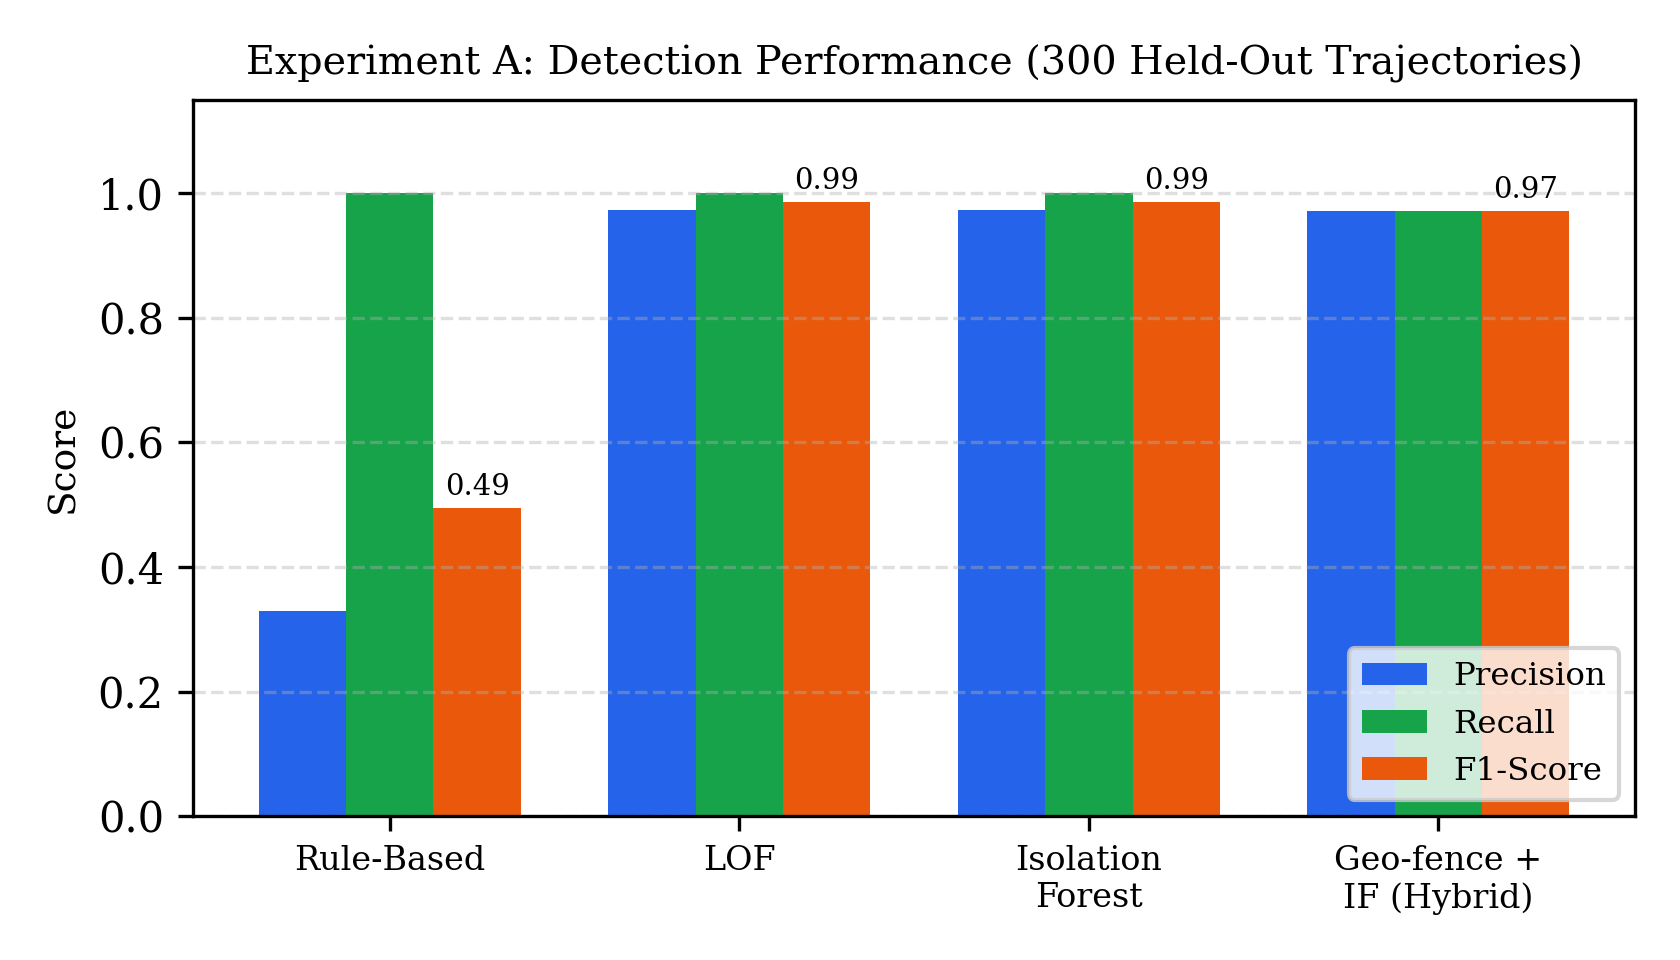
\includegraphics[width=\columnwidth]{figures/fig2_model_comparison.png}
\caption{Experiment A precision, recall, and F1-score across rule-based, LOF, Isolation Forest, and hybrid detectors.}
\label{fig:exp_a}
\end{figure}

\subsection{Experiment B: GPS Error and Jump Sensitivity}
As shown in Table~\ref{tab:exp_b} and Fig.~\ref{fig:exp_b}, the hybrid detector tolerated 30\% missing GPS fixes (F1 = 0.9910, 0.21 false alerts/hr) and stayed effective at 2--5~m noise (F1 = 0.8235--0.8352). At 10--15~m error or 15\% jump spikes, raw position jitter inflated apparent speeds and route deviations, pushing false alerts to 10.60--29.61 per tourist-hour. Urban-canyon deployments should therefore apply Hampel or Kalman smoothing before feature computation.

\begin{table}[t]
\centering
\caption{Experiment B: GPS Noise, Dropout, and Jump Sensitivity}
\label{tab:exp_b}
\scriptsize
\begin{tabular}{@{}lcccccc@{}}
\toprule
\textbf{GPS Condition} & \textbf{FN} & \textbf{FP} & \textbf{Prec.} & \textbf{Rec.} & \textbf{F1} & \textbf{FA/hr} \\
\midrule
2~m GPS error & 0 & 21 & 0.7000 & 1.0000 & 0.8235 & 4.17 \\
5~m GPS error & 11 & 4 & 0.9048 & 0.7755 & 0.8352 & 0.79 \\
10~m GPS error & 14 & 53 & 0.4045 & 0.7200 & 0.5180 & 10.60 \\
15~m GPS error & 0 & 143 & 0.2513 & 1.0000 & 0.4017 & 28.22 \\
Missing GPS (30\%) & 0 & 1 & 0.9821 & 1.0000 & 0.9910 & 0.21 \\
GPS jumps (15\%) & 0 & 150 & 0.2424 & 1.0000 & 0.3902 & 29.61 \\
\bottomrule
\end{tabular}
\end{table}

\begin{figure}[t]
\centering
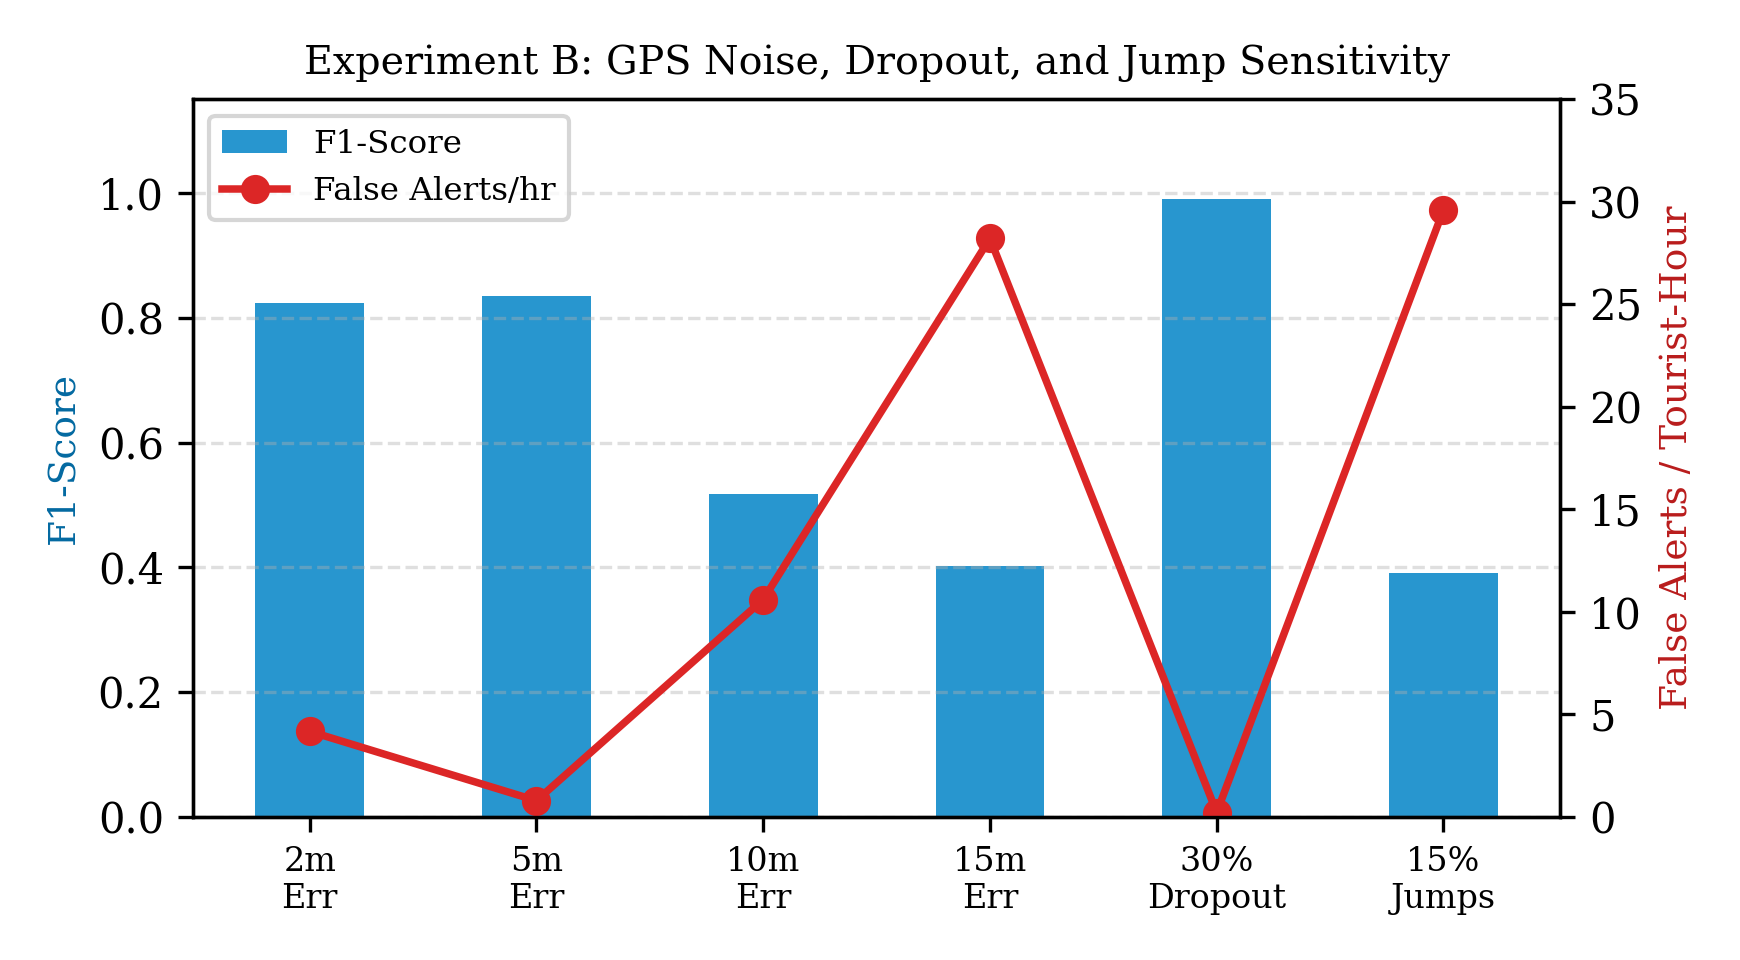
\includegraphics[width=\columnwidth]{figures/fig3_gps_sensitivity.png}
\caption{Experiment B sensitivity of F1-score and false alerts per tourist-hour under degraded GPS conditions.}
\label{fig:exp_b}
\end{figure}

\subsection{Experiment C: Digital Identity Security}
Across 100 trials per case (Table~\ref{tab:exp_c}), 100/100 valid credentials passed in 0.3484~ms on average, while 100/100 modified, expired, revoked, invalid-signature, and replayed presentations were rejected in 0.3415--0.4303~ms. Issuance and ledger anchoring averaged 0.4064~ms across 202 hash-chained blocks with intact chain verification.

\begin{table}[t]
\centering
\caption{Experiment C: Digital Identity Security (100 Trials/Case)}
\label{tab:exp_c}
\scriptsize
\begin{tabular}{@{}lcccc@{}}
\toprule
\textbf{Test Case} & \textbf{Total} & \textbf{Accepted} & \textbf{Rejected} & \textbf{Avg Latency (ms)} \\
\midrule
Valid credential & 100 & 100 & 0 & 0.3484 \\
Modified payload & 100 & 0 & 100 & 0.4302 \\
Expired credential & 100 & 0 & 100 & 0.3964 \\
Revoked on ledger & 100 & 0 & 100 & 0.3415 \\
Invalid issuer sig. & 100 & 0 & 100 & 0.3825 \\
Replayed nonce & 100 & 0 & 100 & 0.4303 \\
\bottomrule
\end{tabular}
\end{table}

\subsection{Experiment D: End-to-End Workflow and Throughput}
Across 20 live HTTP + WebSocket cycles (Table~\ref{tab:exp_d}), restricted-zone entry reached the authority WebSocket client in 137.37~ms on average (582.57~ms P95), and full acknowledgement and closure took 222.05~ms. Under 10 concurrent threads using SQLite and synchronous 24-point Isolation Forest scoring, throughput measured 8.23~req/s (1132.53~ms mean latency), indicating that high-concurrency deployments should enable PostgreSQL/PostGIS pooling and async task queues.

\begin{table}[t]
\centering
\caption{Experiment D: Live Workflow Latency and API Throughput}
\label{tab:exp_d}
\scriptsize
\begin{tabular}{@{}lc@{}}
\toprule
\textbf{Measured System Metric} & \textbf{Observed Value} \\
\midrule
Completed live HTTP + WS workflows & 20 \\
Avg detection-to-WebSocket alert delay & 137.37 ms \\
P95 detection-to-WebSocket alert delay & 582.57 ms \\
Avg end-to-end resolution cycle time & 222.05 ms \\
Concurrent telemetry (100 req, 10 workers) & 8.23 req/s \\
Mean / P95 telemetry API response time & 1132.53 / 1402.34 ms \\
\bottomrule
\end{tabular}
\end{table}

\section{Limitations and Future Work}
First, Experiments A and B rely on synthetic trajectories; consent-based field traces are needed to capture real tourist sightseeing and transit variety. Second, Experiment B highlights sensitivity to 10--15~m GPS error and jump spikes, motivating a Hampel or Kalman filter prior to feature extraction. Third, Experiment C benchmarked our local permissioned ledger state machine rather than a multi-node Hyperledger Fabric Raft cluster, where consensus latency will exceed sub-millisecond local checks. Finally, multi-hour Android field tests are needed to quantify battery consumption under continuous GPS and cellular handoffs.

\section{Conclusion}
We implemented and evaluated a six-module Smart Tourist Safety Monitoring and Incident Response System combining Kotlin mobile telemetry, FastAPI/PostGIS services, Haversine and polygonal geo-fencing, unsupervised movement-anomaly detection, Ed25519 + SHA-256 permissioned identity anchoring, and a React/OpenStreetMap authority dashboard. Automated Python, Android, and React builds pass, and controlled 10-seed trajectory-split evaluations establish F1-scores of $0.9956 \pm 0.0032$ (LOF) and $0.9677 \pm 0.0110$ (Isolation Forest) versus $0.5108 \pm 0.0267$ for static rules, alongside 100\% rejection across five credential attack vectors on our local ledger and 137.37~ms average live WebSocket alert delivery.

\section*{Acknowledgement}
The authors thank the Department of Computer Science and Engineering, K. S. Rangasamy College of Technology (Autonomous), Tiruchengode, Tamil Nadu, India, for academic support and laboratory facilities.

\begin{thebibliography}{00}
\bibitem{aliperti2020} G. Aliperti and A. M. Cruz, ``Promoting built-for-disaster-purpose mobile applications: An interdisciplinary literature review to increase their penetration rate among tourists,'' \textit{J. Hosp. Tour. Manag.}, vol. 44, pp. 193--210, 2020.
\bibitem{chiranjeevi2026} K. Chiranjeevi \textit{et al.}, ``IoT-based smart tourist safety monitoring system,'' \textit{Int. Res. J. Eng. Technol.}, vol. 13, no. 8, 2026.
\bibitem{george2024} B. George, ``Towards safer journeys: Exploring the potential of AI in tourism security,'' \textit{Int. J. Saf. Secur. Tour. Hosp.}, 2024.
\bibitem{premananthan2024} P. Premananthan \textit{et al.}, ``Machine learning applications in smart tourism: Overview, research challenges, and the road ahead,'' \textit{EAI Endorsed Trans. Tour. Technol. Intell.}, 2024.
\bibitem{li2026} Z. Li \textit{et al.}, ``Tourism risk prediction and influencing factor analysis on the Qinghai--Tibet Plateau based on interpretable machine learning,'' \textit{ISPRS Int. J. Geo-Inf.}, vol. 15, no. 5, Art. no. 220, 2026.
\bibitem{josephi2026} A. K. Josephi and M. Maqsood, ``A smart dashboard framework for urban tourism risk analysis using deep learning and machine learning,'' \textit{STAP J. Secur. Risk Manag.}, vol. 2026, no. 1, pp. 112--129, 2026.
\bibitem{hakyemez2025} T. C. Hakyemez and B. Badur, ``Enhancing deep learning-based crime hotspot predictions with theory-based environmental risk scores,'' \textit{Appl. Spat. Anal. Policy}, 2025.
\bibitem{sasaki2024} I. Sasaki \textit{et al.}, ``Data-driven geofencing design for point-of-interest notifiers utilizing genetic algorithm,'' \textit{ISPRS Int. J. Geo-Inf.}, vol. 13, no. 6, Art. no. 174, 2024.
\bibitem{belhadi2020} A. Belhadi \textit{et al.}, ``Trajectory outlier detection: Algorithms, taxonomies, evaluation, and open challenges,'' \textit{ACM Trans. Intell. Syst. Technol.}, vol. 11, 2020.
\bibitem{chandola2009} V. Chandola, A. Banerjee, and V. Kumar, ``Anomaly detection: A survey,'' \textit{ACM Comput. Surv.}, vol. 41, no. 3, 2009.
\bibitem{ali2025} A. Ali \textit{et al.}, ``An innovative IoT and edge intelligence framework for monitoring elderly people using anomaly detection on data from non-wearable sensors,'' \textit{Sensors}, vol. 25, Art. no. 1735, 2025.
\bibitem{mazzocca2025} C. Mazzocca \textit{et al.}, ``A survey on decentralized identifiers and verifiable credentials,'' \textit{IEEE Commun. Surv. Tutor.}, vol. 27, no. 6, pp. 3641--3671, 2025.
\bibitem{muhle2018} A. M\"uhle \textit{et al.}, ``A survey on essential components of a self-sovereign identity,'' \textit{Comput. Sci. Rev.}, vol. 30, 2018.
\bibitem{soltani2021} R. Soltani, U. T. Nguyen, and A. An, ``A survey of self-sovereign identity ecosystem,'' \textit{arXiv:2111.02003}, 2021.
\bibitem{figueroa2021} S. Figueroa-Lorenzo, J. A\~norga Benito, and S. Arrizabalaga, ``Modbus access control system based on SSI over Hyperledger Fabric blockchain,'' \textit{Sensors}, vol. 21, Art. no. 5438, 2021.
\bibitem{akhison2025} G. Akhison, ``Towards a universal digital identity: A blockchain-based framework for borderless verification,'' \textit{Front. Blockchain}, vol. 8, 2025.
\bibitem{khairnar2025} S. Khairnar, ``Application of blockchain frameworks for decentralized identity and access management of IoT devices,'' \textit{IJACSA}, vol. 16, no. 6, 2025.
\bibitem{mountije2025} Y. Mountije, D. Agapito, and C. Ramos, ``Reshaping the future of tourism and hospitality industry through blockchain technology: A systematic literature review,'' \textit{Inf. Technol. Tour.}, vol. 27, pp. 317--343, 2025.
\bibitem{prados2023} J. F. Prados-Castillo \textit{et al.}, ``A review of blockchain technology adoption in the tourism industry from a sustainability perspective,'' \textit{J. Theor. Appl. Electron. Commer. Res.}, vol. 18, no. 2, pp. 814--830, 2023.
\bibitem{rana2022} R. L. Rana, N. Adamashvili, and C. Tricase, ``The impact of blockchain technology adoption on tourism industry: A systematic literature review,'' \textit{Sustainability}, vol. 14, Art. no. 7383, 2022.
\bibitem{zyskind2015} G. Zyskind, O. Nathan, and A. Pentland, ``Decentralizing privacy: Using blockchain to protect personal data,'' in \textit{Proc. IEEE Secur. Privacy Workshops}, 2015.
\end{thebibliography}

\end{document}
